\documentclass[a4paper,10pt]{report}
\usepackage[utf8]{inputenc}
\usepackage{listings}
\usepackage[T1]{fontenc}
\usepackage{graphicx}
% Title Page
\title{Rapport CPA}
\author{Memmi Sacha \\ Shokoufeh}


\begin{document}
\maketitle

\clearpage
\chapter{Préambule}
Les tests que nous avons effectués ont été fait sur une machine possédant 16 Go de RAM ainsi qu'un processeur cadencé à 3.8 Ghz et muni de 12 cores.
\\
Nous avons pu effectuer, au cours de nos recherches, plusieurs implémentations différentes (utilisant différentes structures) dans le but d'optimiser au maximum nos temps d'exécution. 
\newline 

\chapter{Présentation de nos structures de données}
Nous avons utilisé deux structures de données afin de stocker nos graph en mémoire.
\\
Il y a d'une part adjmatrix qui contient une matrice d'incidence. Elle est pratique car elle est assez intuitive à utiliser. Cependant, dès que le graph que nous utilisons est grand est qu'il n'est pas fortement connexe, cette structure doit être dépréciée au profit de la seconde structure de donneé.
\\
La seconde structure de donnée est la structure adjlist. Cette structure contient un tableau qui indique les degrés cumulés de chaque noeud. 
\\
Chaque extrémité d'une arête peut être retrouvée à l'aide de la matrice adj et du tableau des degrés précedemment introduit.
\\
Les deux structures possèdent deux attributs qui sont, e et n, qui donnent respectivement le nombre d'arête de notre graph ainsi que le nombre de noeuds.
\chapter{Construction et stockage de nos données}
\section{Calcul de la taille du graph}
La fonction readEdgeList nous permet de mettre en mémoire notre graph depuis un fichier stocké. 
\\
Le nombre de noeuds est déjà un attribut de notre structure de données. 
\\Par conséquent, nous n'avons pas besoin de le recalculer, il est fait en même temps que la mise en mémoire de notre graph.

Ci dessous, un tableau donnant le nombre d'arêtes et de noeuds pour différents sets de données ainsi que leur temps d'exécution:
\\

\begin{center}
    \begin{tabular}{|l|c|c|c|}
    \hline
     & nodes & edges & Execution time \\ \hline
     Email & 1005 & 25571 & 0s \\
     Amazon & 548 552 & 925775 & 0s\\
     liveJournal & 4 036 538 & 34 681 046 & 20s\\
     orkut & - & - & non calculé \\
     friendster & - & - & non calculé\\
     \hline
    \end{tabular}
\end{center}
Nous pouvons constater avec le tableau ci-dessus, que dès lors que le graph grandit il devient plus délicat de le mettre en mémoire. \\ 
D'où l'absence de certain résultats.
\\
\section{Nettoyage de nos données}
Afin de nettoyer nos données nous avons utilisé la commande linux suivante :
\begin{lstlisting}
 awk '{if ($1<$2) print $1" "$2;else if ($2<$1) print $2" "$1}' net.txt | sort -n -k1,2 -u > net2.txt
\end{lstlisting}
Celle-ci, permet qu'un noeud ne soit relié qu'à un sommet plus grand que lui dans notre fichier. 
\\
Ainsi, les arêtes ne seront prises en compte qu'une fois. 
\\ 
De plus, cette ligne de commande permet de trier suivant l'extrémité de départ d'un edge puis suivant l'extrémité terminale et supprime les doublons.
\\
\section{Les trois différentes datastructures}
Comme nous le disions dans le préambule, nous préférons travailer avec la structure de données adjacency array plutôt que adjancy matrix. 
\\
\newline
En effet, adjacency matrix stock toutes les arêtes possibles (même celles qui n'existent pas), c'est un gâchis d'espace mémoire dans le cas où notre graph est peu dense et que nous n'avons pas besoin de le modifier.
\\
Nous avons pu expérimenter l'importance de la scalabilité de notre structure de données tout au long de nos recherches.
\\
\newline
Nous permettant ainsi, de remarquer le manque de scalabilité de la structure de données adjacency matrix.
\\
\section{Breadth First Search}
\subsection{Structure de données utilisée}
La structure que nous avons utilisé est l'adjacency array car nous n'avions pas besoin de faire des changements dans notre graph.
\\
Nous avons créée une fifo pour visiter tous les noeuds du graph connexe. 
\subsection{Analyse théorique de la complexité temporelle}
La complexité temporelle théorique est O(\textbf{S+A}). Nous parcourons toutes les arêtes ainsi que tous les noeuds

\section{Diamètre}
\subsection{Structure de données utilisée et sous-structure}
Pour déterminer le diamètre de notre graph, nous avons tout d'abord déterminer la taille de ainsi que les noeuds appartenant à la composante connexe la plus grande.
\\
Nous effectuons NDIAMETER fois la boucle suivante 
\\
Ensuite, nous avons déterminé la distance maximale venant d'un noeud aléatoire de cette composante connexe.
\\
Nous prenons le maximum des valeurs retournées dans notre boucle.
\\
Nous avons donc pris le maximum des distances maximales de NDIAMETER tirés aléatoirement parmis ceux nons visités.
\\
\subsection{Analyse de la complexité théorique}
Ici, ce qui sera le plus coûteux dans notre algorithme sera de repérer la composante connexe maximale. 
\\
\newline
En effet, nous allons devoir faire un bfs sur chaque composante connexe.
\\
Nous aurons dans le pire des cas, une complexité en O(\textbf{U * L*log(L)}).
\newline
U étant le nombre de composantes connexes et L le nombre de noeud de cette composante connexe.
\subsection{Analyse expérimentale}
fjdd
\newline
Nous avons pu obtenir les temps d'exécution suivants pour un nombre de noeuds NDIAMETER fixé à 100
\begin{center}
    \begin{tabular}{|l|c|}
    \hline
     Set de données & temps d'exécution\\ \hline
     Email & 1s\\ 
     Amazon & 55s\\ 
     Orkut & 4m52s \\
     Live Journal & 3\\ 
     Friendster & 3\\ 
     \hline
    \end{tabular}
\end{center}
METTRE DIAGRAMME


\section{Détection de triangles}
\subsection{Structure utilisée}
Pour la détection de triangles, nous avons utilisé la structure de données adjacency array car celle-ci convenait le mieux à notre problème.
\\
\subsection{Analyse théorique de la complexité temporelle}
Dans le pire des cas nous effectuons $n^{3}$ comparaisons si tous les noeuds de notre graph sont connectés.
\\
Autrement dit si notre graph forme une unique clique. Ce qui est un cas très rare. 
\\
En général, nous travaillons sur des graphes moyennement connexe. 
\\
Ce qui nous permet d'obtenir une complexité moyenne bien meilleure ainsi que des temps d'exécution tout à fait intéressant comme nous le verrons dans la section consacrée à l'analyse expérimentale.
\\
\newline
En moyenne, nous aurons une complexité en O(\textbf{$S*L^2$}). 
\\
Avec S le nombre de noeuds et L le nombre moyen de voisins d'un noeud.
\clearpage
\subsection{Analyse expérimentale}
Ci-dessous les résultats obtenus.
\newline
\begin{center}
    \begin{tabular}{|l|c|c|}
    \hline
     Set de données & nombre de triangles détectés& temps d'exécution\\ \hline
     Email & 104 333& 0s\\ 
     Amazon &667 129& 1s\\ 
     Orkut & 627584181& 1h35m38 \\
     Live Journal &177820130 & 4m53s\\ 
     Friendster & & 3\\ 
     \hline
    \end{tabular}
\end{center}
Pour le transivity ratio : faire transitivity ratio 
URGENT
\chapter{Détection de communautés dans un graph non orienté}
\section{Génération de graph jouet}
Pour la génération d'un graph, nous prenons en argument un nombre de noeuds un nombre de clusters, un p et un q.
\\
Nous effectuons une séparation simple de nos noeuds en clusters en fonction du nombre de clusters donnés en argument.
\\
Un noeud est relié à un autre noeud du même cluster avec une probabilité p.
\\
Un noeud est relié à un autre noeud d'un cluster différent avec une probabilité q.
\newline
\newline
Lorsque nous augmentons p nous augmentons la connexité au sein d'une même communauté.
\\
À contrario, augmenter q rend la discrimination de communautés plus difficile car il rend les communauté du graph nouvellement créé moins facilement identifiable.
\section{label propagation}
Nous avons effectué une implémentation de l'algorithme de label propagation qui attribue à un sommet le label le plus fréquent dans ses voisins.
\\
Pour ce faire, nous avons utilisé la structure adjmatrix car cela nous semblait plus simple et que nous travaillions sur des graphes jouets plus modestes.
\subsection{Analyse de la complexité théorique}
La fonction highest\_density fait dans le pire des cas 1 fois S comparaison plus 3 fois S comparaisons pour la deuxième boucle. 
\\
Nous conservons une complexité linéaire O(A).
\\
Avec A le nombre d'arêtes de notre graph.
\\
Le core de label\_propagation est une boucle qui itére sur tous les sommets et leur applique highest\_density.
\\
Par conséquent nous avons une complexité en O($S*A$).

\subsection{Analyse expérimentale / Simple Benchmark}
Nous obtenons les résultats suivants:
\\
Les tests ont été effectués avec un p fixé à 0.5. C'est à dire que un noeud a 50 pourcents de chances d'être connecté à un noeud du même cluster. 
Nous fixons le nombre de clusters à 8 et le nombre de noeuds à 400.
\\
Nous obtenons les résultats suivants :\\

 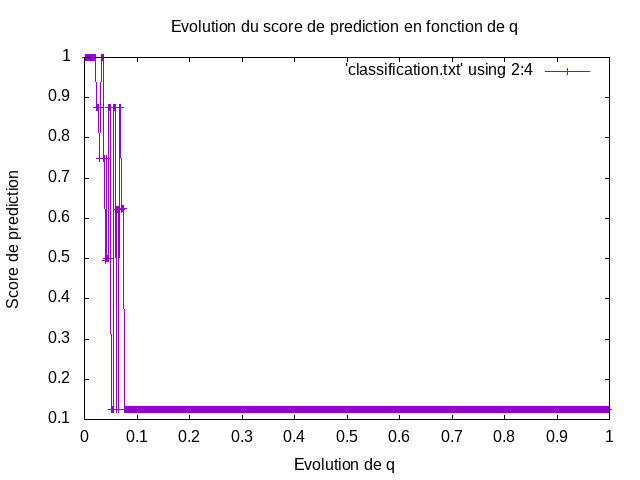
\includegraphics[scale=0.6]{Datas/classificationp05scorelabelpropagation.png}
Nous constatons que notre score de prédiction diminue très rapidement lorsque q augmente. 
\\
Ce qui est logique, car plus q augmente plus nous diminuons notre capacité de distinction entre les communautés.
\\
Pour q = 0.036
\\
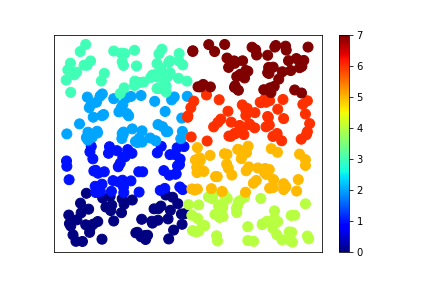
\includegraphics[scale=0.6]{Datas/colorLabelPropagation036.png}
\\
Pour q = 0.04
\\
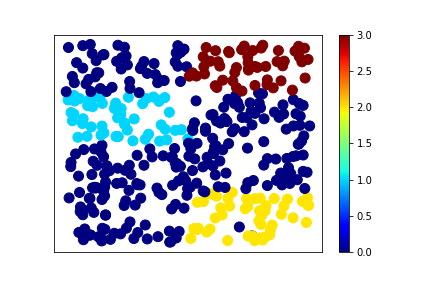
\includegraphics[scale=0.6]{Datas/colorLabelPropagation040.png}
Nous constatons ici qu'il commence à y avoir des chevauchements entre les vraies communautés et les communautés détectées.
\\
Nous avons vérifié, notre algorithme renvoie des résultats corrects lorsque le graph est extrêmement grand.
\section{Algorithme de Jaccard}
Nous avons choisi d'implémenter un label propagation basé sur l'indice de Jaccard. 
\\
\newline
Pour rappel, l'indice de Jaccard permet de calculer la similarité entre les voisins de deux noeuds distincts.
\\
sa formule est donnée par :
\\
\begin{center}
$S(v_i,v_j) = \frac{ T_{v_i} \cap T_{v_j} }{T_{v_i} \cup T_{v_j}}$
\end{center}
Dans notre algrithme, nous utilisons deux fois l'indice de Jaccard. 
\\
Une fois pour déterminer la similarité entre deux noeuds dans le but trier nos noeuds dans l'ordre de similarité du plus grand vers le plus petit.
\newline
La seconde fois où nous utilisons l'indice de Jaccard c'est pour connaître la similarité entre un noeud et une communauté.
\newline
Ce calcul constitue la partie la plus fondamentale de notre algorithme.
\clearpage
\subsection{Analyse expérimentale}
Nous avons conservé le même procédé pouvoir comparer l'efficacité de nos différents algorithmes.
\\
Nous avons donc toujours un p fixé à .5, un nombre de noeuds fixé à 400 ainsi qu'un nombre de clusters fixé à 8.
Nous obtenons le graph suivant :
\newline
\\
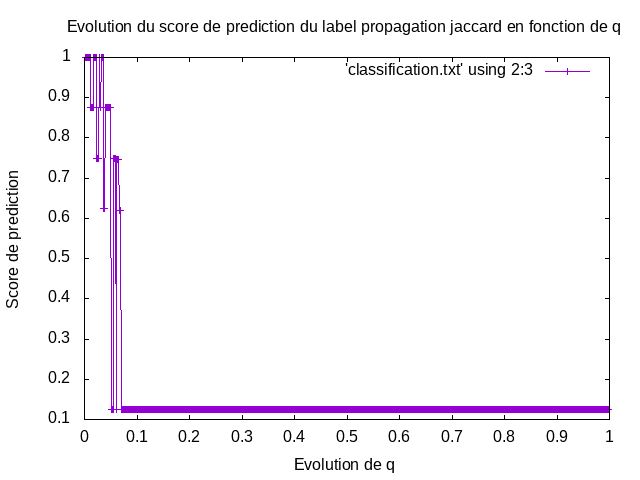
\includegraphics[scale=0.6]{./Datas/classificationp05ScoreJaccard.png}
\\
Nous voyons que notre algorithme donne à peu près les mêmes résultats que le label propagation que nous avons mentionné précedemment.
\\
Cependant, il est tout de même moins stable dans ses résultats.
\section{Louvain personnel}
Nous avons aussi codé un label propagation de Louvain cependant il n'est absolument pas robuste.
\\
Voici les résultats obtenus pour q=.15
\\
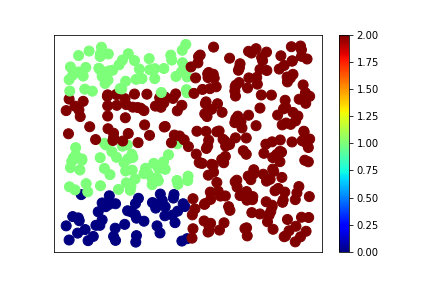
\includegraphics[scale=0.6]{./Datas/colorLouvain015.png}
\section{Comparaisons des trois algorithmes}
Nous superposons les graphes de tous nos résultats:
\\
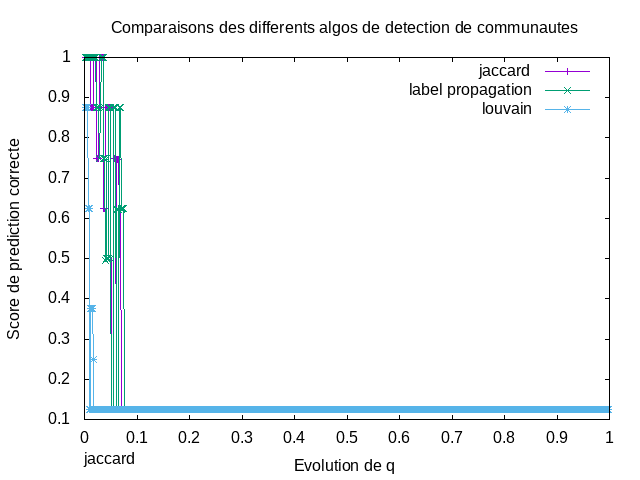
\includegraphics[scale=0.6]{./Datas/compareDetectionsAlgos.png}
Nous remarquons que nos deux algorithmes précedents étaient bien plus efficace que le Louvain que nous avons implémenté.
\\
\section{Experimental Evaluation du louvain fourni}
\end{document}          
